\part{Postludio}
\chapter{Conclusioni}
\begin{figure}[thp]
\centering
\subfloat[][\textit{Architettura di Apex. \parencite{art:apex}}]{\label{subfig:apexarch}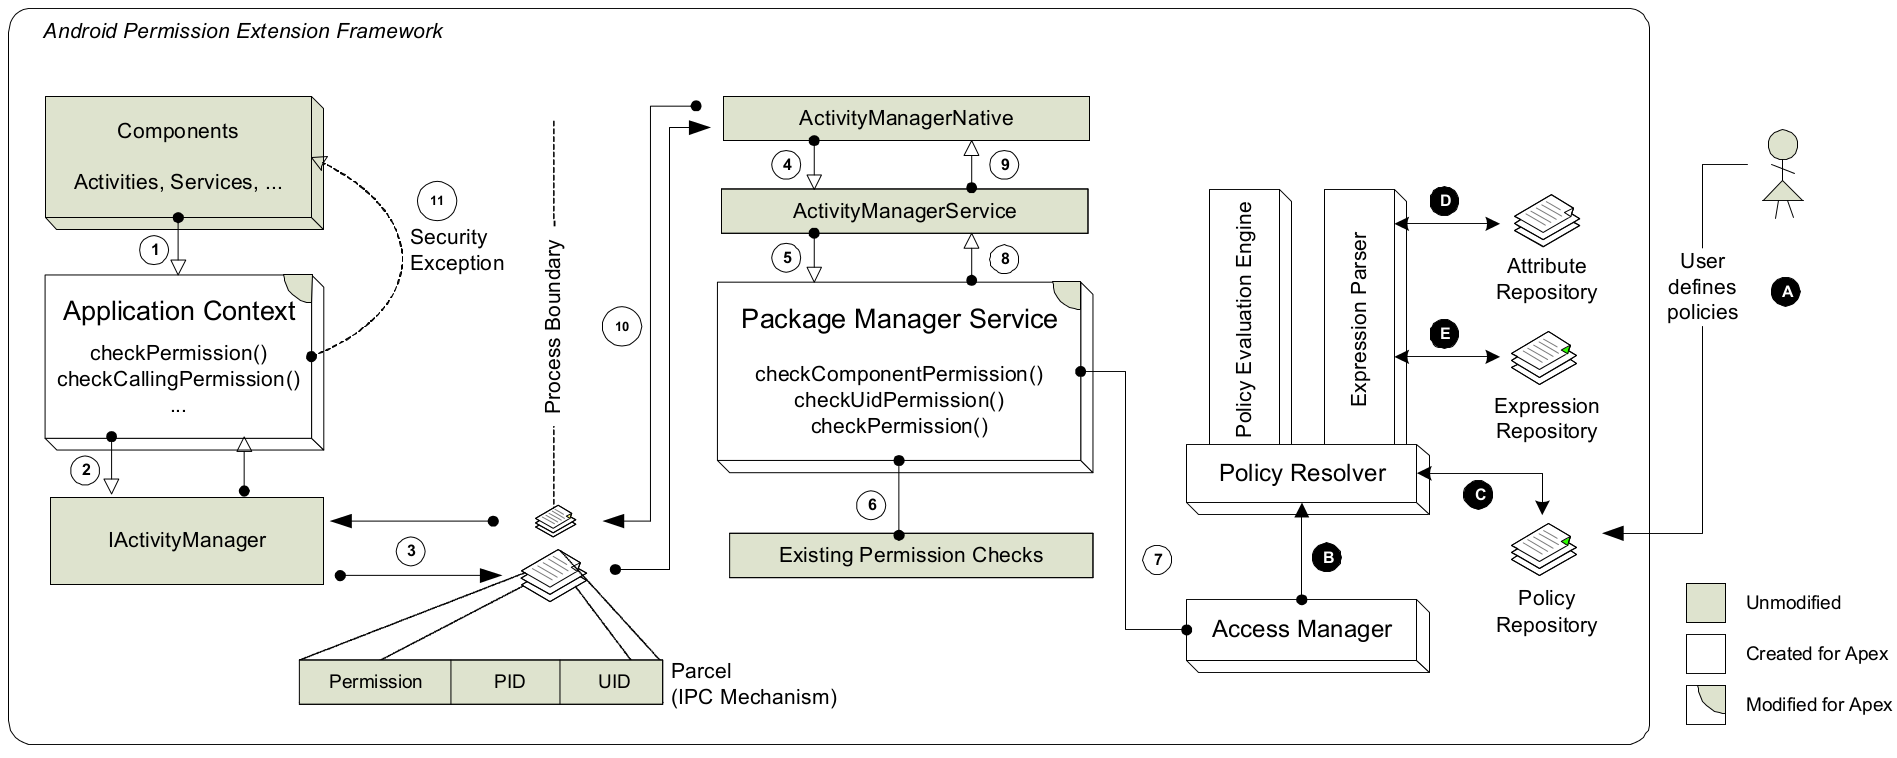
\includegraphics[scale=0.25]{img/conclusioni/apexarch.png}}\\
\subfloat[][\textit{Architettura di Saint. \parencite{art:middleware}}]{\label{subfig:middleware}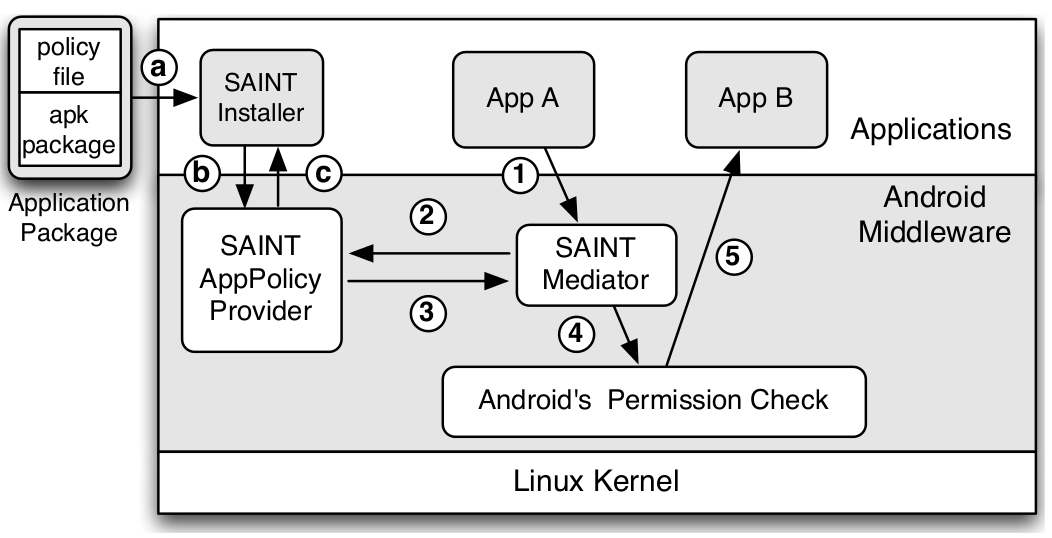
\includegraphics[scale=0.24]{img/conclusioni/saint.png}}\\
\caption{Alcune soluzioni proposte per la gestione dei permessi.}
\label{fig:conclarchfig}
\end{figure}

Dopo aver effettuato molte osservazioni durante la trattazione della presente
Tesi, è necessario puntualizzare ciò che è stato rilevato predisponendo soluzioni
future per il porting di applicazioni all'interno di Android.
\begin{enumerate}
\item L'utilizzo di \textit{upsyscall} delle librerie predisposte all'interno dei
	sistemi Android rende necessaria una riscrittura delle stesse: ritengo
	infatti troppo ardito scoprire a forza di porting di applicativi
	quali siano gli effettivi controlli che vengono effettuati, allo scopo di 
	modificare i sorgenti già esistenti. Con ciò non voglio assolutamente
	affermare che l'effettivo \textit{patching} delle librerie già messe a disposizione
	sia assolutamente inutile, in quanto mette altresì in luce le caratteristiche
	del sistema trattato, ma come questa sia una strada che richiederebbe
	l'impiego di un tempo considerevole. 
	
	In Figura \vref{fig:conclarchfig} voglio riassumere brevemente quali
	altri sistemi sono stati studiati per modificare le politiche di controllo dei
	processi a livello di servizi:
	\subref{subfig:apexarch} si potrebbe modificare l'implementazione degli stessi
	o \subref{subfig:middleware} inserire un ulteriore strato intermedio.
\item Considerando le osservazioni effettuate nella Sottosezione \vref{subsec:mischeWilhelm},
	posso mostrare come si potrebbe ampliare questo lavoro di tesi tramite
	la creazione di un servizio intermedio (in linguaggio C++ o Java),
	il quale implementi la politica di caching per la fruizione del sampling
	audio.
	
	Una possibile politica implementativa sarebbe quella tramite la gestione
	di produttori-consumatori (utilizzando nel caso specifico un solo
	produttore) a buffer limitato, implementando in questo modo una politica
	di caching. A questo punto sarebbe necessario riscrivere la libreria
	Wilhelm, in modo da effettuare l'interazione non più con \texttt{\small 
	AudioFlinger} ma con questo nuovo \textit{service} che si contrapporrebbe
	a quest'ultimo. 
	
	Un'eventuale approccio sarebbe quello di inserire tale politica all'interno
	del codice stesso di Android: con questa soluzione non sarebbe necessario
	modificare l'interazione della libreria Wilhelm, ma si riscontrerebbe
	una maggior difficoltà in quanto si dovrebbe modificare un codice molto
	intricato.
	
	Sebbene inizialmente si sarebbe portati a rimuovere drasticamente l'interazione
	tra librerie e \textit{service} Android poiché questi spesso causano una limitazione
	nell'esecuzione degli applicativi (vedi nella gestione dei permessi),
	detto \textit{middleware} si rivela utile in quanto viene predisposto un
	meccanismo di IPC che sarebbe interessante estendere allo scopo di 
	evadere le stesse limitazioni, emerse nella trattazione.
	
	Non sarebbe tuttavia possibile implementare questo meccanismo all'interno
	di Pjproject, in quanto ciò consentirebbe solamente ad applicazioni
	di tale progetto di ottenere i benefici perseguiti, ed inoltre tale
	scelta implicherebbe l'implementazione di un meccanismo per il quale
	tali programmi debbano ottenere informazioni condivise tra processi.
\item Un ulteriore aspetto che reputerei interessante indagare sul sistema
	operativo Android sarebbe la creazione dei \textit{service} Java lato utente
	utilizzando le API predisposte e di come questi possano interagire
	con il device Binder. Immediatamente legato a quest'aspetto è collegato
	il meccanismo con il quale si effettua il \textit{launch} di un'applicazione
	Java.
\item Una grossa difficoltà da me riscontrata nella redazione di questa tesi 
	è dovuta alla presenza di interessanti informazioni in lingua Cinese,
	che però non conosco. Nelle fasi iniziali ho provato ad effettuare traduzioni
	sommarie tramite l'utilizzo di traduttori automatici, che tuttavia
	si sono rivelati inutili per documentazioni complesse, discorsive ed
	articolate, ma che hanno stuzzicato ulteriormente la mia curiosità.
\end{enumerate}
